\documentclass[a4paper,10pt]{article}

\usepackage{graphicx}
\usepackage{polyglossia}

\usepackage[hyphens]{url}
\usepackage{hyperref}
\usepackage{fontspec}
\setmainfont{Source Serif Pro}
\setsansfont{Source Sans Pro}


\usepackage{hyperref}


\setdefaultlanguage[spelling=new,babelshorthands=true]{german}

\usepackage[left=2cm,right=2cm,top=3.0cm,bottom=3.0cm]{geometry}


\title{
	Projekt Assembler-Programmierung \\
	SNAKE
}
\author{
	\Large Marc Uxa \& Benjamin Huber \\[2mm]
	\texttt Jahrgang: 18-INB2 \& 19-INB1 \\
	\normalsize HTWK Leipzig \\
}
\date{\today}

\begin{document}
	\maketitle
	% \mbox{}\hrule\mbox{}
	\thispagestyle{empty}
	\newpage
	
	\setcounter{page}{1}
	\tableofcontents
	\newpage
	
	\section{Spiel}
		\subsection{Anleitung}
			
			Bei diesem Spiel handelt es sich um das klassische Snake-Spiel. Es 
			muss 
			Futter eingesammelt werden, bei jedem Einsammeln steigt der Score 
			um einen Punkt.\\
			Es kann zwischen verschiedenen Schwierigkeitsgraden gewählt werden. 
			Je nach Modus ändert sich die Geschwindigkeit und die Punkteanzahl 
			die benötigt wird um das Spiel erfolgreich zu beenden. Die Stufen 
			können mit einem Mausklick auf des entsprechende Word ausgewählt 
			werden.\\
			%
			easy (mode = 1):
			\begin{itemize}
				\item[-] speed = 4
				\item[-] max. 30 Punkte erreichbar
				\item[-] ab 15 Punkten erhöht sich die Geschwindigkeit 
			\end{itemize}
			%
			normal (mode = 2):
			\begin{itemize}
				\item[-] speed = 3
				\item[-] max. 40 Punkte erreichbar
				\item[-] ab 20 Punkten erhöht sich die Geschwindigkeit 
			\end{itemize}
			%
			hard (mode = 3):
			\begin{itemize}
				\item[-] speed = 2
				\item[-] max. 50 Punkte erreichbar
				\item[-] ab 35 Punkten erhöht sich die Geschwindigkeit 
			\end{itemize}
			%
			Die Schlange kann mit den folgenden Tasten gesteuert werden:
			\begin{itemize}
				\item[-] W nach oben
				\item[-] A nach links
				\item[-] S nach unten
				\item[-] D nach rechts
			\end{itemize}
			Mit ESC kann das Spiel sofort beendet und geschlossen werden.
			%
		\subsection{Besonderheiten}
			In dem Programm sind diese Teile enthalten:
			\begin{itemize}
				\item[-] eigene Interrupt Service Routine für ISR1Ch
				\item[-] eigene Maus Unterroutine (AH = 0Ch)
				\item[-] Videomodus 3 (VGA-Grafik)
				\item[-] Soundeffekte
			\end{itemize}
		\newpage
		%
	\section{Entwurfsskizzen}
		
		\subsection{Programmlogik}
			Die Prozedur "resetSnake" \- aktualisiert unser Schlangen-Array und 
			wird vor jedem Zeichnen aufgerufen. Dabei werden die Werte in dem 
			Array von der höchsten zur niedrigsten Stelle, jeweils um ein Feld 
			verschoben. \\
			Bei "snakeInc" \- wird eine nicht initialisierte Feld (mit 0 
			beschriebenes Feld) mit einem Wert beschrieben und somit wird 
			eine verlängerte Schlange gezeichnet. \\
			\begin{figure}[h]
				\centering
				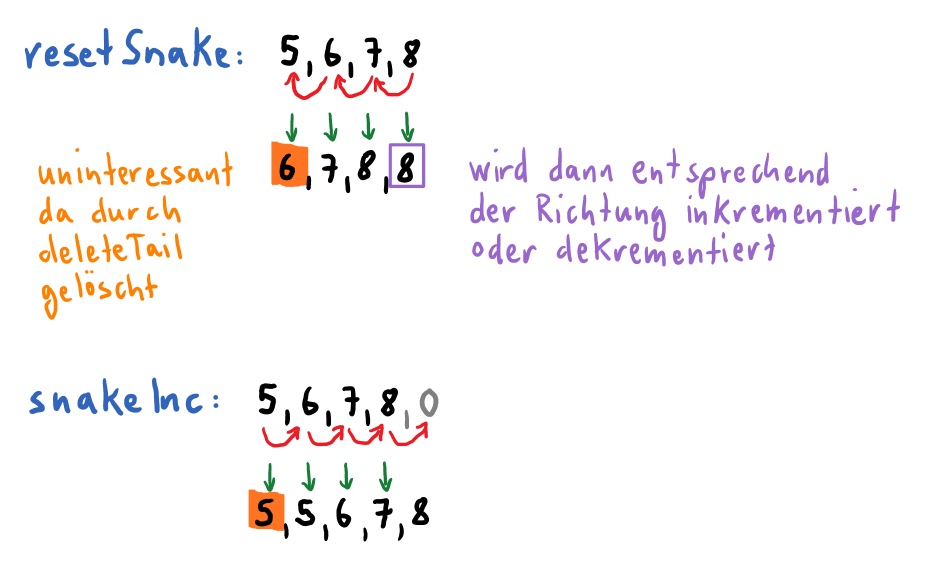
\includegraphics[width=0.65\textwidth]{prog}
				\caption{Prozeduren resetSnake und snakeInc}
				\label{SnakPro}
			\end{figure}
			%
			
			Das nachfolgende Bild zeigt, wie die Koordinaten angepasst werden, 
			je nach Richtung in der sich die Schlange bewegen soll.\\
			\begin{figure}[h]
				\centering
				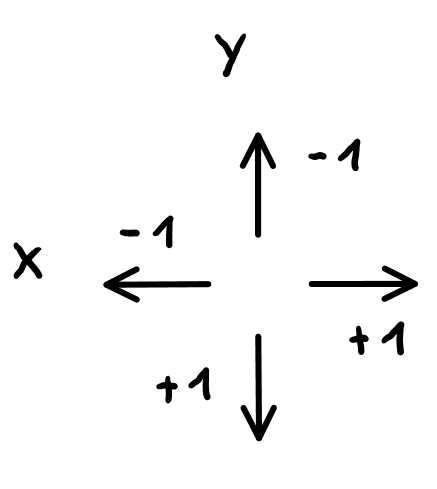
\includegraphics[width=0.45\textwidth]{richtung}
				\caption{Bewegung der Schalnge}
				\label{move}
			\end{figure}
			%
			\newpage
		\subsection{GUI Skizzen}
			Die grafische Oberfläche wurde nach den nachfolgenden Skizzen 
			erstellt:\\
		
			\begin{figure}[h]
				\centering
				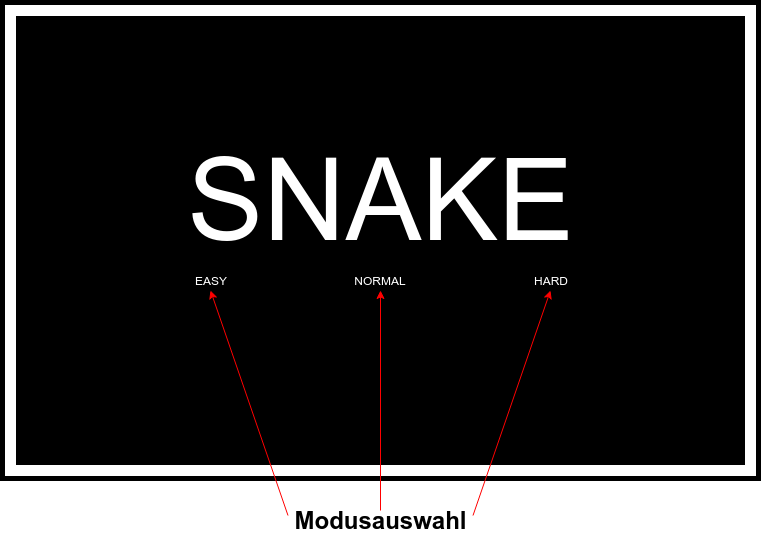
\includegraphics[width=0.65\textwidth]{GUI_start}
				\caption{Startbildschirm}
				\label{GUI-Start}
			\end{figure}
			%
			\begin{figure}[h]
				\centering
				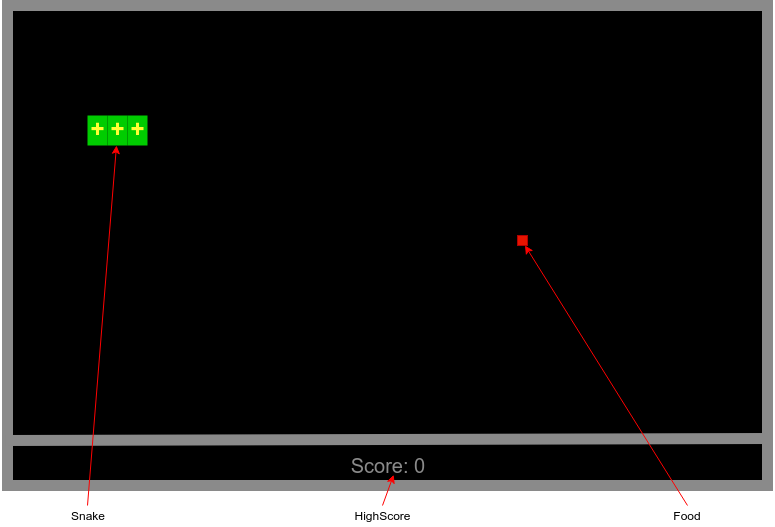
\includegraphics[width=0.65\textwidth]{GUI_SKizze-gameplay}
				\caption{Spielbildschirm}
				\label{GUI-Gameplay}
			\end{figure}
			\newpage
			%
			\begin{figure}[h]
				\centering
				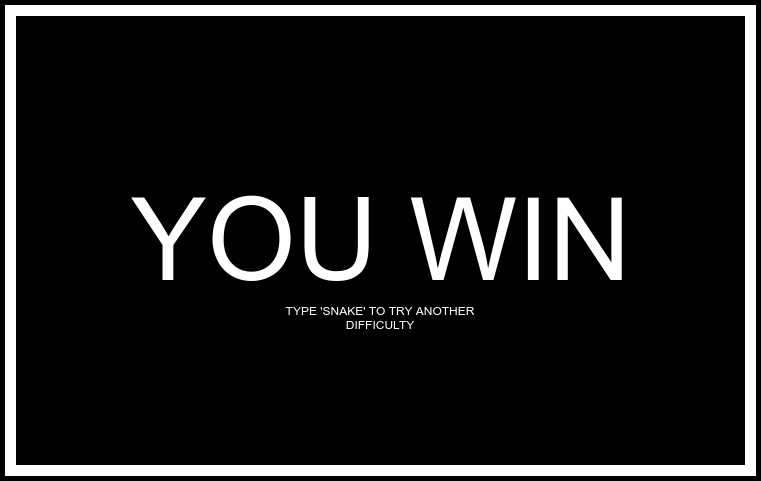
\includegraphics[width=0.65\textwidth]{GUI_SKizze-win}
				\caption{Bildschirm bei erfolgreichem Spielende}
				\label{GUI-Win}
			\end{figure}
			%
			\begin{figure}[h]
				\centering
				
\includegraphics[width=0.65\textwidth]{GUI_SKizze-lose}
				\caption{Bildschirm bei verlorener Runde}
				\label{GUI-Lose}
			\end{figure}
			\newpage
			%
	\section{Programmarchitektur}
		Nach dem untenstehenden Diagramm ist die Architektur aufgebaut: \\
		\begin{figure}[h]
			\centering
			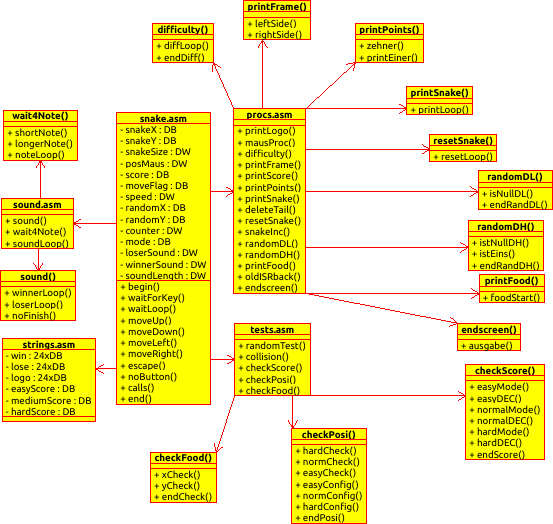
\includegraphics[width=1\textwidth]{Klassendiagramm}
			\caption{Programmstruktur}
			\label{UML}
		\end{figure}
		%
		
		Es gibt eine snake.asm Datei, in der die Steuerung des Rundenablaufs, 
		sowie die Auswahl des härte Grades implementiert ist. Dabei nutzt das 
		Hauptprogramm andere ASM-Dateien in denen verschiedene Prozeduren für 
		die Tonausgabe und die einzelnen Bauteile für den Spielablauf enthalten 
		sind. In einer weiteren Datei sind die Zeichenketten, für den 
		Startbildschirm und für die zwei möglichen Endbildschirme gespeichert.\\
		\newpage
		%
	\section{Tests}
		\subsection{Random Numbergenerator Test 1}
			
			Die Test der Zufallszahlen würde in einer Tabelle festgehalten.\\
			\begin{figure}[h]
				\centering
				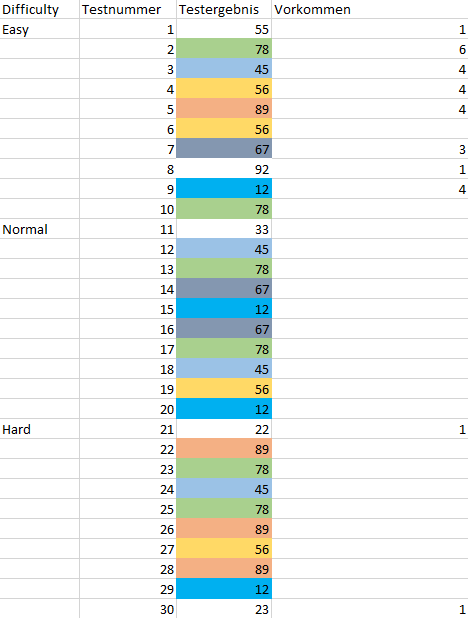
\includegraphics[width=0.65\textwidth]{tests}
				\caption{RNG Test 1}
				\label{RNG1}
			\end{figure}
			%
			
			Wie man an der Tabelle erkennen kann wiederholen sich immer wieder 
			dieselben Zahlen in anderer Reihenfolge. Es handelt sich also 
			hierbei nur um einen Pseudozufallszahlengenerator (PRNG). Am Anfang 
			kommen (meist) die selben beiden Zahlen raus was daran liegt, dass 
			es durch die "sound" \- - Prozedur keine Verzögerung gibt, welche 
			man 
			aber brauch, damit andere Zahlen rauskommen. Der Unterschied durch 
			die "sound" \- - Prozedur ist auch sehr gering und berechenbar. Im 
			Allgemeinen funktionieren die Zahlen, aber da wir bei 30 Tests 10 
			Unterschiedliche Zahlen bekommen und dies reicht, damit das 
			Zeichnen des Futters zufällig wirkt.
			\newpage
			%
		\subsection{Random Numbergenerator Test 2}
		
			Nachdem wir in diesem Test das kleine Delay durch die "sound" \- - 
			Prozedur nicht mehr ausnutzen kommen immer 2-mal dieselben Zahlen 
			raus, 
			jedoch im Gesamten viel mehr unterschiedliche Zahlen, weshalb wir 
			uns entscheiden, diese Methode beizubehalten, weil es so auch 
			optisch schöner im Gesamtbild ist.
			\begin{figure}[h]
				\centering
				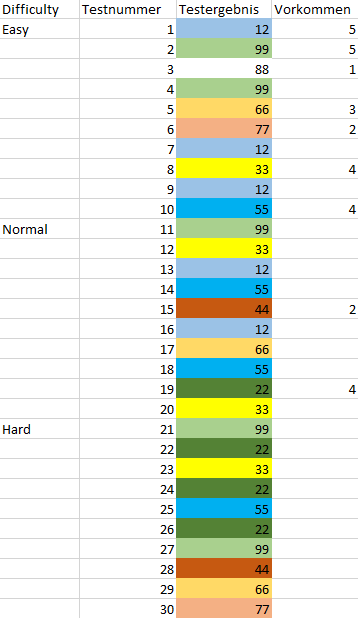
\includegraphics[width=0.55\textwidth]{tests_2}
				\caption{RNG Test 2}
				\label{RNG2}
			\end{figure}
			\newpage
			%
		\subsection{Collision Test}
		
			In dieser Prozedur wird überprüft ob der Schlangenkopf mit einem 
			anderen "+" \- Zeichen kollidiert, ist das der Fall berührt sich 
			die 
			Schlange selber und das Spiel ist vorbei.
			%
		\subsection{Check Score}
		
			Hier wird überprüft ob die vorgegebene Punktezahl erreicht ist mit 
			der ein Spiel gewonnen wird oder die Geschwindigkeit erhöht wird.
			%
		\subsection{Check Posi}
		
			Wird überprüft ob ein Buchstabe der Strings "easy", "normal" \- 
			oder 
			"hard" \- angeklickt wurde und setzt die entsprechende 
			Konfiguration 
			in dem Spiel.
			%
		\subsection{Check Food}
		
			Testet ob die Position des Schlangenkopfs mit der Position des 
			Futters übereinstimmt. Sind die Koordinaten die selben, ertönt ein 
			Ton, die Schlange wird verlängert und das Futter wird einer neuen 
			Stelle gezeichnet
			%.
\end{document}